\chapter{最小生成樹}
\label{ch:mst}

% 本章的圖共用的樣式（點、強調的點、邊、選中的邊、要拿掉的邊、權重標籤）
\tikzset{
    mstv/.style={circle, draw=black!60, thick, minimum size=0.7cm, inner sep=0pt, font=\small},
    mstvhl/.style={mstv, draw=memStroke, fill=memFill},
    mstvblue/.style={mstv, draw=coreStroke, fill=coreFill},
    mste/.style={thick, draw=black!35},
    mstehl/.style={line width=1.6pt, draw=memStroke},
    mstenew/.style={line width=1.6pt, draw=memStroke, dashed},
    mstebad/.style={line width=1.6pt, draw=optStroke, dashed},
    mstw/.style={font=\scriptsize, text=black!70, fill=white, inner sep=1pt},
    mstnote/.style={font=\scriptsize, text=coreStroke},
}

工業區裡有六座廠房，管委會要鋪光纖把它們連成一個網路。 下圖是可以施工的九條
路線，邊上的數字是造價（萬元）。 訊號可以經過別的廠房轉送，所以不需要每兩座
之間都直接拉線，只要任兩座廠房之間有一條由光纖接起來的路就好。 最少要花多少
錢？ 往下讀之前，先在圖上挑一次，算出你的總造價。

\begin{center}
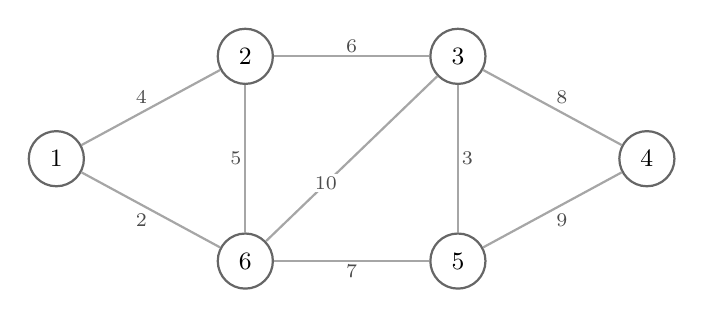
\begin{tikzpicture}[x=1.5cm, y=1.3cm]
\node[mstv] (1) at (0,1) {1};
\node[mstv] (2) at (1.6,2) {2};
\node[mstv] (6) at (1.6,0) {6};
\node[mstv] (3) at (3.4,2) {3};
\node[mstv] (5) at (3.4,0) {5};
\node[mstv] (4) at (5,1) {4};
\draw[mste] (1) -- node[mstw, above left] {4} (2);
\draw[mste] (1) -- node[mstw, below left] {2} (6);
\draw[mste] (2) -- node[mstw, left] {5} (6);
\draw[mste] (2) -- node[mstw, above] {6} (3);
\draw[mste] (6) -- node[mstw, below] {7} (5);
\draw[mste] (3) -- node[mstw, right] {3} (5);
\draw[mste] (3) -- node[mstw, above right] {8} (4);
\draw[mste] (5) -- node[mstw, below right] {9} (4);
\draw[mste] (6) -- node[mstw, pos=0.35] {10} (3);
\end{tikzpicture}
\diagcaption{六座廠房和九條可以施工的光纖路線，邊上的數字是造價。}
\label{fig:mst-factories}
\end{center}

六座廠房至少要五條線才連得起來，而且用五條剛好連通時，線路不會繞成圈：多出一
個圈，就表示圈上有一條線拿掉之後大家仍然相通，那條線是白花的錢。 所以答案一定
是一棵連到全部六個點的樹。 從九條裡挑五條有 $126$ 種挑法，其中 $55$ 種剛好連
成一棵樹，最便宜的那一種花 $23$ 萬元。 你挑的是 $23$ 嗎？

這一章講怎麼不靠枚舉，直接找出這棵最便宜的樹：\textbf{Kruskal 演算法}把邊由便宜到
貴排好，能接就接；\textbf{Prim 演算法}從一個點長出一棵樹，每次接上最便宜的往外的
邊。 兩者都是貪心，理由是同一個交換論證。 之後再看三種變形：總和要最大、圖要自己
建、路上最窄的一段要盡量寬（瓶頸問題）。

這一章用到：本書第~7~章的並查集（直接沿用那一章的 \texttt{find} 和
\texttt{unite}，不再重講）；第~8~章的 Dijkstra 演算法和
\texttt{priority\_queue}；《C++ 演算法解題 1：APCS 實作題核心》（以下簡稱第 1 本）
第~7~章的貪心和交換論證；第 1 本第~11~章的邊列表、鄰接串列和 BFS；第 1 本第~13~章
「$n$ 個點的樹剛好有 $n - 1$ 條邊」。

\section{生成樹}
\label{sec:mst-tree}

這一章的圖都是無向圖，每條邊有一個\textbf{權重}（weight），可能代表造價、距離或
時間。 同一對點之間可以有好幾條邊（重邊），權重不一定相同。

一張連通的圖有 $n$ 個點。 從它的邊裡挑出一些，如果挑出來的邊能讓全部 $n$ 個點
彼此相通，而且沒有環，這些邊就叫做這張圖的一棵\textbf{生成樹}（spanning tree）。
「生成」指的是它碰到了每一個點。 第 1 本第~13~章說過，$n$ 個點連通又沒有環，剛好
是 $n - 1$ 條邊，所以生成樹一定是 $n - 1$ 條邊；反過來，挑了 $n - 1$ 條邊又讓全
部的點相通，一定沒有環。

生成樹的權重是它的邊的權重總和。 所有生成樹裡權重最小的，叫\textbf{最小生成樹}
（minimum spanning tree，常簡寫成 MST）。 章首的問題就是求最小生成樹，答案是
$23$。 最小生成樹可能不只一棵，例如權重相同的邊可以互換，但它們的總權重都一樣。

題目通常不會寫「求最小生成樹」，而是寫「選一些路線，讓任兩個地點都能到達，總造價
最小」或「剛好選 $n - 1$ 條，讓全部連通」。 權重都是正的時候，兩種說法是同一件事。
權重可以是負的時候就不一樣：第一種說法裡負的邊選越多越省，答案可能有環；第二種限
定了 $n - 1$ 條，仍然是生成樹。 這一章的例題和題單都屬於第二種，或權重都不是負的。

\subsection{和最短路徑不一樣}
\label{sec:mst-vs-sp}

第~8~章的 Dijkstra 從起點 $s$ 出發，替每個點找出最短的路。 每個點記下最短路上的
前一個點，這 $n - 1$ 條「前一步」的邊合起來也是一棵生成樹，叫\textbf{最短路徑樹}
（shortest-path tree）。 它和最小生成樹看起來很像，都是一棵樹、都在挑便宜的邊，
但兩者照顧的東西不同：

\begin{center}
\begin{tikzpicture}[x=1.3cm, y=1.1cm]
\begin{scope}
\node[font=\small] at (1,2.8) {最短路徑樹：總權重 $18$};
\node[mstvhl] (s) at (0,1) {$s$};
\node[mstv] (a) at (2,2) {$a$};
\node[mstv] (b) at (2,1) {$b$};
\node[mstv] (c) at (2,0) {$c$};
\draw[mstehl] (s) -- node[mstw, above left] {5} (a);
\draw[mstehl] (s) -- node[mstw, above, pos=0.6] {6} (b);
\draw[mstehl] (s) -- node[mstw, below left] {7} (c);
\draw[mste] (a) -- node[mstw, right] {2} (b);
\draw[mste] (b) -- node[mstw, right] {2} (c);
\node[mstnote, right=0.25cm] at (a.east) {距離 5};
\node[mstnote, right=0.25cm] at (b.east) {距離 6};
\node[mstnote, right=0.25cm] at (c.east) {距離 7};
\end{scope}
\begin{scope}[xshift=6cm]
\node[font=\small] at (1,2.8) {最小生成樹：總權重 $9$};
\node[mstvhl] (s) at (0,1) {$s$};
\node[mstv] (a) at (2,2) {$a$};
\node[mstv] (b) at (2,1) {$b$};
\node[mstv] (c) at (2,0) {$c$};
\draw[mstehl] (s) -- node[mstw, above left] {5} (a);
\draw[mste] (s) -- node[mstw, above, pos=0.6] {6} (b);
\draw[mste] (s) -- node[mstw, below left] {7} (c);
\draw[mstehl] (a) -- node[mstw, right] {2} (b);
\draw[mstehl] (b) -- node[mstw, right] {2} (c);
\node[mstnote, right=0.25cm] at (a.east) {距離 5};
\node[mstnote, right=0.25cm] at (b.east) {距離 7};
\node[mstnote, right=0.25cm] at (c.east) {距離 9};
\end{scope}
\end{tikzpicture}
\diagcaption{同一張圖上，從 $s$ 出發的最短路徑樹（左）和最小生成樹（右）。 粗線是
樹上的邊，藍字是沿著樹從 $s$ 走過去的距離。}
\label{fig:mst-vs-spt}
\end{center}

左邊的最短路徑樹讓\textbf{每個點到 $s$ 的距離}都最短，總權重 $18$；右邊的最小生成
樹讓\textbf{邊的總和}最小，只要 $9$，代價是 $c$ 沿著樹走離 $s$ 有 $9$，直接走只要
$7$。 想像 $s$ 是機房：要省鋪線的錢選右邊，要每台機器到機房的延遲最小選左邊。 另
外，最小生成樹沒有起點，最短路徑樹換一個起點就整棵不同。

暴力解是枚舉所有 $n - 1$ 條邊的組合，用第~7~章的並查集檢查有沒有環，留下權重最小
的。 章首的圖只有 $\binom{9}{5} = 126$ 種組合；$m = 30$、$n = 16$ 時已經大約
$1.6 \times 10^8$ 種，$m$ 到 $2 \times 10^5$ 完全不可能。 它寫起來不難，留著當對拍用。

\section{Kruskal 演算法}
\label{sec:kruskal}

最便宜的線應該盡量用。 照這個直覺，先試兩條看起來合理的規則，都拿章首的圖來試。

\begin{itemize}
\item \textbf{規則 A：直接拿最便宜的 $n - 1$ 條。} 最便宜的五條是 $2, 3, 4, 5, 6$，
也就是 1--6、3--5、1--2、2--6、2--3。 其中 1--2、2--6、1--6 繞成一個三角形，
廠房 4 卻一條線都沒接到。
\item \textbf{規則 B：每座廠房各自選一條連出去最便宜的線。} 1 選 1--6、2 選
1--2、3 和 5 都選 3--5、4 選 3--4、6 選 1--6，合起來是四條線，分成
$\{1, 2, 6\}$ 和 $\{3, 4, 5\}$ 兩塊，接不起來。
\end{itemize}

規則 A 的問題出在三角形：2--6 這條線接上的兩座廠房，早就經由 1 相通了，它沒有
幫上任何忙，還佔掉了一個名額。 把這一點修好，就是 Kruskal 演算法：

\begin{itemize}
\item 把所有的邊依權重由小到大排好。
\item 依序看每一條邊 $(u, v)$：如果 $u$ 和 $v$ 目前還不相通，就選它；如果早就相
通，選它只會繞成環，跳過。
\item 選滿 $n - 1$ 條就完成了。
\end{itemize}

「目前相不相通」正是第~7~章並查集在做的事：\texttt{unite(u, v)} 回傳
\texttt{true} 表示兩群原本分開、現在合併了，這條邊就要選；回傳 \texttt{false}
表示早就同一群，跳過。

\subsection{在章首的圖上跑一次}

九條邊排序之後依序處理，每一列是一條邊：

\begin{center}
\begin{tabular}{cclll}
\toprule
邊 & 權重 & 兩端 & 結果 & 處理完的群 \\
\midrule
1--6 & 2 & 不同群 & 選 & $\{1, 6\}$ $\{2\}$ $\{3\}$ $\{4\}$ $\{5\}$ \\
3--5 & 3 & 不同群 & 選 & $\{1, 6\}$ $\{2\}$ $\{3, 5\}$ $\{4\}$ \\
1--2 & 4 & 不同群 & 選 & $\{1, 2, 6\}$ $\{3, 5\}$ $\{4\}$ \\
2--6 & 5 & 同一群 & 跳過 & 不變 \\
2--3 & 6 & 不同群 & 選 & $\{1, 2, 3, 5, 6\}$ $\{4\}$ \\
6--5 & 7 & 同一群 & 跳過 & 不變 \\
3--4 & 8 & 不同群 & 選 & $\{1, 2, 3, 4, 5, 6\}$ \\
5--4 & 9 & 同一群 & 跳過 & 不變 \\
6--3 & 10 & 同一群 & 跳過 & 不變 \\
\bottomrule
\end{tabular}
\end{center}

選到 1--6、3--5、1--2、2--3、3--4 五條，總和 $2 + 3 + 4 + 6 + 8 = 23$，畫出來就是
下一節圖~\ref{fig:mst-cut} 的右半邊。 注意 6--5 雖然只要 $7$，比 3--4 的 $8$ 便宜，
卻被跳過了：它要接的兩座廠房早就經由 6--1--2--3--5 相通。

\subsection{程式}

輸入第一行是 $n$、$m$，接著 $m$ 行「$u$ $v$ $w$」。 邊存成邊列表（第 1 本第~11~
章），因為 Kruskal 只需要把邊排序，用不到鄰接串列。 程式印出選到的每一條邊和總
和；圖不連通時印出 \texttt{disconnected}。

\begin{example}[label=ex:mst-kruskal]{cpp}{(kruskal.cpp) Kruskal 演算法}
#include <algorithm>
#include <iostream>
#include <utility>
#include <vector>
using namespace std;

struct Edge {
    int u, v;
    long long w;
};

vector<int> parent, sz;

int find(int x) {
    return parent[x] == x ? x : parent[x] = find(parent[x]);
}

bool unite(int a, int b) {
    a = find(a);
    b = find(b);
    if (a == b) {
        return false;
    }
    if (sz[a] > sz[b]) {
        swap(a, b);
    }
    parent[a] = b;
    sz[b] += sz[a];
    return true;
}

int main() {
    int n, m;
    cin >> n >> m;
    vector<Edge> edges(m);
    for (Edge &e : edges) {
        cin >> e.u >> e.v >> e.w;
    }
    sort(edges.begin(), edges.end(),
         [](const Edge &a, const Edge &b) { return a.w < b.w; });
    parent.resize(n + 1);
    sz.assign(n + 1, 1);
    for (int i = 1; i <= n; i++) {
        parent[i] = i;
    }
    long long total = 0;
    int used = 0;
    for (const Edge &e : edges) {
        if (unite(e.u, e.v)) {         // 兩端原本不連通：選
            total += e.w;
            used++;
            cout << e.u << ' ' << e.v << ' ' << e.w << '\n';
        }                              // 否則會繞成環：跳過
    }
    if (used == n - 1) {
        cout << "total " << total << '\n';
    } else {
        cout << "disconnected\n";
    }
    return 0;
}
\end{example}

\iosample{
6 9 \\
1 2 4 \\
1 6 2 \\
2 6 5 \\
2 3 6 \\
6 5 7 \\
3 5 3 \\
3 4 8 \\
5 4 9 \\
6 3 10 \\
}{
1 6 2 \\
3 5 3 \\
1 2 4 \\
2 3 6 \\
3 4 8 \\
total 23 \\
}

\begin{itemize}
\item \texttt{find} 和 \texttt{unite} 和第~7~章修路的程式（\texttt{roads.cpp}）一字
不差：按大小合併加路徑壓縮。 這一章每一支程式都用同一份。
\item 排序用 lambda 只比權重（銜接書第~9~章），權重相同的邊誰先都可以。
\item \texttt{total} 用 \texttt{long long}。 $n$ 到 $2 \times 10^5$、權重到
$10^9$ 時，總和可以到 $2 \times 10^{14}$。
\item \texttt{used} 數選了幾條。 等於 $n - 1$ 時其實可以直接 \texttt{break}，後面
的邊都會被跳過；不寫也一樣對，只是多跑幾次 \texttt{find}。
\end{itemize}

\textbf{複雜度}：排序 $O(m \log m)$，之後 $m$ 次 \texttt{unite}，每次幾乎是常數
時間（第~7~章）。 整體是 $O(m \log m)$，時間幾乎都花在排序上。

\subsection{圖不連通的時候}
\label{sec:mst-forest}

如果圖本身不連通，就沒有生成樹。 Kruskal 照樣可以跑完：每一塊連通元件各自連成
一棵樹，合起來是一片森林，叫做\textbf{生成森林}（spanning forest）；Kruskal 得到
的是總權重最小的那一片。 圖有 $c$ 個連通元件時，森林有 $n - c$ 條邊，所以只要看
選了幾條：少於 $n - 1$ 條就表示不連通。

題目對不連通的要求各有不同：輸出 $-1$、輸出森林的總權重，或問最少還要加幾條線（答
案是 $c - 1$）。 \texttt{used} 和 $c = n - \texttt{used}$ 都在手上，照題目要的輸出就
好。

\subsection{什麼時候用、什麼時候不能用}

\begin{itemize}
\item 適合：「選一些邊讓所有點連通，總權重最小」或「剛好選 $n - 1$ 條讓全部連
通」，邊直接給在輸入裡，$m$ 到 $2 \times 10^5$ 左右。
\item 不能用：\textbf{有向圖}（例如沿著單行道從總部到每個地點），Kruskal 會選出走
不通的方向，這是另一個問題，超出本書範圍。
\item 不能用：\textbf{只要連通其中幾個點}，其他點可經過可不經過。 這叫 Steiner 樹
問題，目前沒有已知的有效率解法，資料量通常很小，只能枚舉。
\end{itemize}

\section{為什麼 Kruskal 是對的}
\label{sec:mst-cut}

第 1 本第~7~章看過很多「看起來合理、其實會錯」的貪心，例如郵票先貼大面額。
Kruskal 每一步只看眼前最便宜的邊，選了就不回頭，也需要一個理由。 這一節用第 1 本
第~7~章的交換論證證明它。 先介紹一個工具。

\subsection{切割}

把圖上的點分成兩邊，一邊叫 $S$，另一邊是其他的點，這樣的分法叫一個\textbf{切割}
（cut）。 一條邊的兩端如果分在不同邊，就說它\textbf{跨過}這個切割。 下圖把章首的
圖切成 $S = \{1, 2, 6\}$ 和 $\{3, 4, 5\}$，跨過去的邊有 2--3、6--5、6--3 三條。

任何一棵生成樹都必須至少用一條跨過的邊，否則 $S$ 裡的點到不了另一邊。 直覺上，
要過去，就從跨過的邊裡挑最便宜的。 這個直覺是對的：

\begin{center}
\fbox{\parbox{0.88\linewidth}{\textbf{切割性質}（cut property）：任取一個切割，跨過
它的邊裡權重最小的那一條 $e$，一定包含在某一棵最小生成樹裡。}}
\end{center}

證明用交換論證。 任取一棵最小生成樹 $T$。 如果 $T$ 裡有 $e$，就證完了。 如果沒
有，設 $e$ 連接 $u$ 和 $v$，$u$ 在 $S$ 裡、$v$ 不在。

\begin{itemize}
\item \textbf{找一條可以換掉的邊。} $T$ 是生成樹，$u$ 到 $v$ 在 $T$ 上有一條路。
這條路從 $S$ 出發、結束在 $S$ 外面，中途一定有某一條邊 $f$ 跨過切割。
\item \textbf{換完仍然合法。} 把 $T$ 加上 $e$、拿掉 $f$，得到 $T'$。 $T'$ 還是
$n - 1$ 條邊。 原本經過 $f$ 的路，都可以改走「$T$ 上那條路剩下的部分，加上
$e$」繞過去，所以 $T'$ 仍然讓全部的點相通，是一棵生成樹。
\item \textbf{換完沒有變差。} $e$ 是跨過切割的邊裡最小的，$f$ 也跨過切割，所以
$e$ 的權重 $\le$ $f$ 的權重，$T'$ 的總權重 $\le$ $T$ 的總權重。 $T$ 已經是最小，
所以 $T'$ 也是最小生成樹，而且包含 $e$。
\end{itemize}

下圖是一個實際的例子。 $T$ 是一棵沒有用到 2--3 的生成樹，總權重 $24$。 加上
2--3 之後，2--3--5--6--1--2 繞成一個環，環上另一條跨過切割的邊是 6--5，把它拿掉，
總權重變成 $24 + 6 - 7 = 23$。

\begin{center}
\begin{tikzpicture}[x=1.05cm, y=1.1cm]
\begin{scope}
\fill[coreFill, rounded corners=8pt] (-0.5,-0.45) rectangle (2.1,2.45);
\node[font=\small, coreStroke] at (0.2,2.7) {$S$};
\node[font=\small] at (2.5,3.1) {$T$，總權重 $24$；加上 $e$};
\node[mstv] (1) at (0,1) {1};
\node[mstv] (2) at (1.6,2) {2};
\node[mstv] (6) at (1.6,0) {6};
\node[mstv] (3) at (3.4,2) {3};
\node[mstv] (5) at (3.4,0) {5};
\node[mstv] (4) at (5,1) {4};
\draw[mstehl] (1) -- node[mstw, above left] {4} (2);
\draw[mstehl] (1) -- node[mstw, below left] {2} (6);
\draw[mstebad] (6) -- node[mstw, below] {$f$: 7} (5);
\draw[mstehl] (3) -- node[mstw, right] {3} (5);
\draw[mstehl] (3) -- node[mstw, above right] {8} (4);
\draw[mstenew] (2) -- node[mstw, above] {$e$: 6} (3);
\end{scope}
\begin{scope}[xshift=7cm]
\fill[coreFill, rounded corners=8pt] (-0.5,-0.45) rectangle (2.1,2.45);
\node[font=\small, coreStroke] at (0.2,2.7) {$S$};
\node[font=\small] at (2.5,3.1) {$T'$，總權重 $23$};
\node[mstv] (1) at (0,1) {1};
\node[mstv] (2) at (1.6,2) {2};
\node[mstv] (6) at (1.6,0) {6};
\node[mstv] (3) at (3.4,2) {3};
\node[mstv] (5) at (3.4,0) {5};
\node[mstv] (4) at (5,1) {4};
\draw[mstehl] (1) -- node[mstw, above left] {4} (2);
\draw[mstehl] (1) -- node[mstw, below left] {2} (6);
\draw[mstehl] (3) -- node[mstw, right] {3} (5);
\draw[mstehl] (3) -- node[mstw, above right] {8} (4);
\draw[mstehl] (2) -- node[mstw, above] {6} (3);
\end{scope}
\end{tikzpicture}
\diagcaption{切割 $S = \{1, 2, 6\}$（藍底）。 左：生成樹 $T$ 加上跨過切割最便宜的
邊 $e$（虛線），形成一個環，環上另一條跨過切割的邊是 $f$（紅色虛線）。 右：拿掉
$f$ 之後的 $T'$。}
\label{fig:mst-cut}
\end{center}

\subsection{Kruskal 每一步都選了切割上最便宜的邊}

現在把切割性質套到 Kruskal 上。 要證明的是下面這句話，對 Kruskal 的每一步都成立：

\begin{center}
目前選到的邊，全部包含在某一棵最小生成樹裡。
\end{center}

一開始一條邊都還沒選，當然成立。 假設選了一些邊之後還成立，設這些邊包含在最小
生成樹 $T$ 裡。 Kruskal 接著選了邊 $e = (u, v)$，取 $S$ 是 $u$ 目前所在的那一群
（並查集裡的那一群），$v$ 不在 $S$ 裡。 這個切割有兩個特點：

\begin{itemize}
\item 已經選的邊都不跨過它。 已選的邊兩端一定在同一群，而 $S$ 剛好是一整群。
\item $e$ 是跨過它的邊裡最便宜的。 理由在下面的框裡。
\end{itemize}

接著照切割性質的證明做交換：$T$ 加上 $e$ 形成的環上，有另一條跨過切割的邊 $f$，
換掉它得到 $T'$。 因為已選的邊都不跨過切割，被換掉的 $f$ 不會是已選的邊，所以
$T'$ 仍然包含所有已選的邊，再加上 $e$。 這句話在選了 $e$ 之後仍然成立。

一直到選滿 $n - 1$ 條，選到的邊包含在某一棵最小生成樹裡，而它們本身就有
$n - 1$ 條，所以它們就是那一棵最小生成樹。 這和第 1 本第~7~章交換論證的三步對得
起來：任取一個最佳解；把和貪心不一樣的地方換成貪心的選擇，仍然合法、沒有變差；
每換一次，最佳解和貪心相同的邊就多一條，所以會停。

\begin{whybox}[$e$ 是跨過 $S$ 最便宜的邊]
看任何一條比 $e$ 便宜、而且跨過 $S$ 的邊 $g = (x, y)$。 Kruskal 依權重由小到大處
理，$g$ 比 $e$ 先處理過。 處理 $g$ 的時候只有兩種可能：

\begin{itemize}
\item $x$、$y$ 不同群：Kruskal 會選 $g$，兩群合併，$x$、$y$ 從此在同一群。
\item $x$、$y$ 已經同群：群只會合併、不會拆開，從此也一直在同一群。
\end{itemize}

兩種情況下，現在 $x$ 和 $y$ 都在同一群，不可能一個在 $S$ 裡、一個在外面，和「$g$
跨過 $S$」矛盾。 所以跨過 $S$ 的邊沒有比 $e$ 便宜的。 和 $e$ 一樣便宜的邊可能有，
這不影響證明：切割性質只要求 $e$ 不比其他跨過的邊貴。 這也說明了權重相同的邊誰
先處理都可以。
\end{whybox}

\subsection{環性質}

切割性質還有一個反過來的版本，第~\ref{sec:mst-build}~節建圖時會用到：

\begin{center}
\fbox{\parbox{0.88\linewidth}{\textbf{環性質}（cycle property）：如果一條邊 $h$ 在某
個環上，而且比環上其他每一條邊都\textbf{嚴格}重，$h$ 不會出現在任何一棵最小生成
樹裡。}}
\end{center}

理由也是交換：假設某棵最小生成樹 $T$ 用了 $h$。 把 $h$ 拿掉，$T$ 分成兩塊。 那個
環從 $h$ 的一端繞回另一端，路上一定有另一條邊 $g$ 連接這兩塊。 用 $g$ 換掉 $h$ 得
到的仍然是生成樹，而 $g$ 比 $h$ 輕，總權重嚴格變小，和 $T$ 最小矛盾。

在章首的圖上，6--3（權重 $10$）在環 6--3--5--6 上，比 3--5（$3$）和 6--5（$7$）都
重，所以不管怎麼選，最小生成樹都不會用它。 Kruskal 跳過的每一條邊，其實都是這種
「環上最重」的邊：它被跳過時兩端已經經由更便宜的邊相通，那條路加上它就是一個環。

如果所有的邊權重都不相同，用環性質可以證明最小生成樹只有一棵（本章練習第~2~
題）。 有相同權重時可能有好幾棵，但總權重都一樣。

\section{Prim 演算法}
\label{sec:prim}

Kruskal 一次看整張圖，同時長出好幾小塊，最後才接成一棵。 Prim 演算法換一個方向：
從一個點開始，只維護\textbf{一棵}樹，每一步把「一端在樹上、另一端還不在」的邊裡
最便宜的那條接上，樹就多一個點。 接了 $n - 1$ 次，全部的點都在樹上。

它為什麼對？ 每一步的 $S$ 取「目前在樹上的點」，要接的邊正是跨過這個切割最便宜
的那一條，已經選的邊都在 $S$ 裡面、不跨過切割，所以上一節的論證整段可以照搬。

\subsection{和 Dijkstra 長得很像}

要很快找出「往外最便宜的邊」，就把往外的邊放進 \texttt{priority\_queue}。 寫出
來和第~8~章的 Dijkstra 幾乎一樣，只差在堆裡放的數字：從 $u$ 往 $v$ 的邊，Dijkstra
放 $\mathrm{dist}[u] + w$（經過 $u$ 到 $v$ 的距離），Prim 只放 $w$（把 $v$ 接到樹上
的費用）。 只差這一點，結果就是圖~\ref{fig:mst-vs-spt} 左右兩棵不同的樹。 寫 Prim 時
最常見的錯誤，就是順手把 Dijkstra 的 \texttt{dist[u] + w} 抄了過來。

章首的圖從點 1 開始，堆裡的元素寫成（費用，點）：

\begin{center}
\begin{tabular}{clll}
\toprule
步 & 從堆裡拿出 & 結果 & 新放進堆的 \\
\midrule
1 & (0, 1) & 1 上樹 & (4, 2)、(2, 6) \\
2 & (2, 6) & 6 上樹，費用 2 & (5, 2)、(7, 5)、(10, 3) \\
3 & (4, 2) & 2 上樹，費用 4 & (6, 3) \\
4 & (5, 2) & 2 已經在樹上，丟掉 & \\
5 & (6, 3) & 3 上樹，費用 6 & (3, 5)、(8, 4) \\
6 & (3, 5) & 5 上樹，費用 3 & (9, 4) \\
7 & (7, 5) & 5 已經在樹上，丟掉 & \\
8 & (8, 4) & 4 上樹，費用 8 & \\
\bottomrule
\end{tabular}
\end{center}

之後堆裡剩下的 (9, 4)、(10, 3) 拿出來都會丟掉。 費用加起來 $2 + 4 + 6 + 3 + 8 =
23$，選到的邊和 Kruskal 相同，只是順序不一樣：Kruskal 照權重由小到大選，Prim 照
點上樹的順序選，第 5、6 步先花 $6$ 再花 $3$。 費用 $3$ 的 3--5 一直到 3 上樹之後
才「往外」，在那之前它兩端都不在樹上，Prim 看不到它。

\begin{code}{cpp}{Prim 演算法的主迴圈（用 priority\_queue）}
// adj[u]：(鄰居, 權重) 的鄰接串列，點 1 到 n
vector<bool> inTree(n + 1, false);
priority_queue<pair<long long, int>, vector<pair<long long, int>>,
               greater<pair<long long, int>>> pq;   // (費用, 點)，小的在頂端
pq.push({0, 1});                        // 從點 1 開始，接進來不用錢
long long total = 0;
int count = 0;
while (!pq.empty()) {
    auto [w, u] = pq.top();
    pq.pop();
    if (inTree[u]) {                    // 已經在樹裡：過期的紀錄
        continue;
    }
    inTree[u] = true;
    total += w;
    count++;
    for (auto [v, wv] : adj[u]) {
        if (!inTree[v]) {
            pq.push({wv, v});
        }
    }
}
// count < n 表示圖不連通
\end{code}

\begin{itemize}
\item 同一個點可能被放進堆好幾次（表裡的點 2 就有兩筆），只有第一次拿出來的那筆
最便宜，之後的都是過期的紀錄，用 \texttt{inTree} 檢查後丟掉。 這和第~8~章
Dijkstra 丟掉過期紀錄的「先不刪」寫法相同。
\item \texttt{inTree[u] = true} 一定要寫在\textbf{拿出來}的時候，不能寫在放進去的
時候。 放進去時只表示「有一條路可以接到 $u$」，不代表那是最便宜的一條（本章練習
第~4~題）。
\item Prim 只會長出點 1 所在的那一棵樹。 圖不連通時，\texttt{count} 會小於 $n$。
要的是生成森林的話，對每一個還不在樹上的點再開始一次。
\end{itemize}

\textbf{複雜度}：每條邊最多讓兩筆紀錄進堆，堆的操作共 $O(m)$ 次，每次
$O(\log m)$，整體 $O(m \log m)$，和 Kruskal 一樣。

\subsection{稠密圖：不用堆的 Prim}
\label{sec:prim-dense}

有一類題目，任兩個點之間都可以連線，費用由兩點的位置算出來，例如「$n$ 根旗桿，
任兩根都能拉線，費用是兩根的曼哈頓距離 $|x_i - x_j| + |y_i - y_j|$」。 這種圖有
$n(n - 1)/2$ 條邊，邊數是點數平方的量級，叫\textbf{稠密圖}（dense graph）；邊數和點
數差不多的叫\textbf{稀疏圖}（sparse graph）。

$n = 5000$ 時有 $12497500$ 條邊。 Kruskal 要先把這一千兩百多萬條邊全部存下來再排
序；用堆的 Prim 也會把同樣多的紀錄塞進堆裡。 Prim 有一個更簡單的寫法：替每個還
不在樹上的點記一個數 \texttt{best[v]}，表示「把 $v$ 接到目前這棵樹上最少要多少
錢」。 每一步：

\begin{itemize}
\item 掃過所有不在樹上的點，挑 \texttt{best} 最小的 $u$，讓它上樹。
\item 掃過所有不在樹上的點 $v$，算出 $u$ 到 $v$ 的費用 $d$，如果 $d$ 比
\texttt{best[v]} 小，就更新。 $u$ 剛上樹，所以「接到樹上」多了一個選擇。
\end{itemize}

每一步是兩次 $O(n)$ 的掃描，做 $n$ 步，總共 $O(n^2)$。 邊的費用需要時才算，完全
不用存邊。

\begin{code}{cpp}{稠密圖的 Prim，$O(n^2)$：點 $0$ 到 $n - 1$，座標存在 x、y}
vector<long long> best(n, INF);         // 接到目前這棵樹的最低費用
vector<bool> inTree(n, false);
best[0] = 0;
long long total = 0;
for (int round = 0; round < n; round++) {
    int u = -1;
    for (int i = 0; i < n; i++) {       // 樹外 best 最小的點
        if (!inTree[i] && (u == -1 || best[i] < best[u])) {
            u = i;
        }
    }
    inTree[u] = true;
    total += best[u];
    for (int v = 0; v < n; v++) {       // u 上樹之後，更新其他點
        if (!inTree[v]) {
            long long d = llabs(x[u] - x[v]) + llabs(y[u] - y[v]);
            best[v] = min(best[v], d);
        }
    }
}
\end{code}

例如五根旗桿在 $(0, 0)$、$(2, 2)$、$(3, 10)$、$(5, 2)$、$(7, 0)$，最小生成樹是
$(2,2)$--$(5,2)$（$3$）、$(0,0)$--$(2,2)$（$4$）、$(5,2)$--$(7,0)$（$4$）、
$(2,2)$--$(3,10)$（$9$），總和 $20$。

在本書測試的環境下，$n = 5000$ 個隨機的點，這個寫法（補上讀入和輸出）約 $0.04$ 秒，記憶體約
$3$ MB。 把全部 $12497500$ 條邊存下來跑 Kruskal，得到同樣的答案，但要約
$0.72$ 秒和約 $199$ MB，記憶體已經超過很多題目的限制。 輸入直接給一個
$n \times n$ 的鄰接矩陣（第 1 本第~11~章）時，也是同樣的情況，用這個寫法最省事。

\subsection{選哪一個}

Kruskal 和用堆的 Prim 都是 $O(m \log m)$，前者用邊列表，後者用鄰接串列。 大部分題
目用 Kruskal 就好，它最短，也最容易延伸到後面幾節的變形。 看到「任兩點都可以連」而
且 $n$ 只有幾千，或輸入是鄰接矩陣，改用 $O(n^2)$ 的 Prim。 如果 $n$ 到 $10^5$ 又任
兩點都能連，兩種都來不及，要先像第~\ref{sec:mst-build}~節那樣，證明大部分的邊用不
到。

\section{最大生成樹}
\label{sec:max-st}

反過來，要總權重\textbf{最大}的生成樹，叫\textbf{最大生成樹}（maximum spanning
tree）。 做法只改一個地方：Kruskal 的邊改成由\textbf{大到小}排序，Prim 改成每次
接最貴的往外的邊。 章首的圖的最大生成樹總和是 $37$。

為什麼這樣就對？ 把每條邊的權重變號，$w$ 變成 $-w$。 每一棵生成樹的總權重也跟著
變號，原本最大的變成最小的，所以「原圖的最大生成樹」就是「變號之後的最小生成
樹」。 而對變號後的圖由小到大跑 Kruskal，正好就是對原圖由大到小跑。 這個論證沒
有用到權重是正的，切割性質的證明也沒有，所以\textbf{權重是負數時 Kruskal 照樣對}，
最大生成樹和最小生成樹都一樣。 要小心的只是題目的說法（第~\ref{sec:mst-tree}~
節）：限定剛好 $n - 1$ 條時，負的邊該選還是要選。

\subsection{例題：學伴配對的最高默契總分}
\label{sec:ex-buddy}

\textbf{題意}（\akiref{best-total-buddy-compatibility}{學伴配對的最高默契總分}）

\begin{itemize}
\item 有 $n$ 位新生，學生會列出 $m$ 組候選配對，第 $i$ 組是新生 $u_i$ 和 $v_i$，
默契分數 $w_i$，可能是負的。 同一對新生可能出現在好幾組裡，分數不一定相同，每
一組都可以單獨選或不選。
\item 要從中挑出\textbf{剛好 $n - 1$ 組}，讓所有新生沿著挑出來的配對串在一起。
\item 輸出挑出來的分數總和最大是多少，負的分數照算。
\item $n \le 10^5$，$m \le 2 \times 10^5$，$|w_i| \le 10^9$。 保證全部選上時所有
新生會串在一起。
\end{itemize}

例如 $4$ 位新生，配對是 $(1, 2)$ 分數 $3$、$(1, 3)$ 分數 $1$、$(2, 3)$ 分數 $-2$、
$(3, 4)$ 分數 $-7$。 新生 4 只出現在 $(3, 4)$ 裡，不選它就接不上，所以一定要選；
剩下兩組選 $3$ 和 $1$，總和 $3 + 1 - 7 = -3$。

\textbf{想法}

暴力解是枚舉 $m$ 組裡選哪 $n - 1$ 組，$\binom{m}{n - 1}$ 種，只在 $m$ 很小時可行。

「剛好 $n - 1$ 組，全部串在一起」就是生成樹的定義，要總分最大，就是最大生成樹。
照上面說的，把配對依分數由大到小排序跑 Kruskal：會讓兩群新生串起來的就選，兩人
已經串在一起的就跳過。 負分的配對不用特別處理：輪到它時如果還有兩群沒串起來，
就表示比它好的配對都接不起這兩群，只能選它。

同一對新生的重複配對也不用特別處理。 分數高的那一組先被看到，如果選了，同一對
後面的配對兩端已經相通，自然會跳過。

同樣的模型也出現在別的地方：幾個倉庫之間要排固定的運輸路線，每條路線一年的淨
收益有正有負，主管規定剛好開 $n - 1$ 條、而且每個倉庫都要接上，要讓總收益最大。

\textbf{程式}

\begin{example}[label=ex:mst-buddy]{cpp}{(buddy.cpp) 學伴配對的最高默契總分}
#include <algorithm>
#include <iostream>
#include <utility>
#include <vector>
using namespace std;

struct Edge {
    int u, v;
    long long w;
};

vector<int> parent, sz;

int find(int x) {
    return parent[x] == x ? x : parent[x] = find(parent[x]);
}

bool unite(int a, int b) {
    a = find(a);
    b = find(b);
    if (a == b) {
        return false;
    }
    if (sz[a] > sz[b]) {
        swap(a, b);
    }
    parent[a] = b;
    sz[b] += sz[a];
    return true;
}

int main() {
    ios::sync_with_stdio(false);
    cin.tie(nullptr);
    int n, m;
    cin >> n >> m;
    vector<Edge> edges(m);
    for (Edge &e : edges) {
        cin >> e.u >> e.v >> e.w;
    }
    sort(edges.begin(), edges.end(),
         [](const Edge &a, const Edge &b) { return a.w > b.w; });  // 大的先
    parent.resize(n + 1);
    sz.assign(n + 1, 1);
    for (int i = 1; i <= n; i++) {
        parent[i] = i;
    }
    long long total = 0;
    for (const Edge &e : edges) {
        if (unite(e.u, e.v)) {
            total += e.w;               // 負分也照加
        }
    }
    cout << total << '\n';
    return 0;
}
\end{example}

\iosample{
5 7 \\
1 2 4 \\
2 3 6 \\
1 3 5 \\
3 4 -2 \\
4 5 3 \\
2 5 1 \\
1 2 2 \\
}{
15 \\
}

\begin{itemize}
\item 和範例~\ref{ex:mst-kruskal} 只差在比較函式的 \texttt{>}，以及不用印出選到的
邊。 題目保證全部選上時會串在一起，所以不用檢查 \texttt{used}。
\item 範例裡依序選了 $6$、$5$、$3$、$1$，跳過第一組 $(1, 2)$ 的 $4$（1、2 已經經
由 3 串在一起）和最後一組 $(1, 2)$ 的 $2$；$-2$ 的 $(3, 4)$ 輪到時，全部的人已經
串在一起，也跳過。 總和 $6 + 5 + 3 + 1 = 15$。
\end{itemize}

\textbf{複雜度}：$O(m \log m)$。 最大的測試資料在本書測試的環境下約 $0.02$ 秒。

\subsection{常見錯誤}

\begin{itemize}
\item \textbf{照抄最小生成樹的排序}：比較函式寫成 \texttt{a.w < b.w}，求出來的是
最小生成樹。 範例 1 印出 \texttt{4}，上面 $4$ 位新生的例子印出 \texttt{-8}。
\item \textbf{只加正分}：寫成 \texttt{if (e.w > 0) total += e.w;}。 範例 1 剛好
沒選到負分，仍然印出正確的 \texttt{15}；$4$ 位新生的例子印出 \texttt{4}，正確答案
是 \texttt{-3}。 「剛好 $n - 1$ 組」時，負分的配對是被迫要選的。
\item \textbf{總和用 \texttt{int}}：$n = 10^5$ 位新生排成一串、每組都是 $10^9$ 分，
正確答案是 \texttt{99999000000000}。 \texttt{total} 改成 \texttt{int}，在本書測試的
環境下印出 \texttt{-723552768}，加了 \texttt{-Wall -Wextra} 也沒有警告。
\end{itemize}

\section{自己建出圖來}
\label{sec:mst-build}

前面的圖都直接寫在輸入裡。 很多題目要自己決定點是什麼、邊是什麼。 第
~\ref{sec:prim-dense}~節的旗桿就是一例：點是旗桿，任兩根之間都有一條邊。 有時候
邊的數量多到存不下，這時要用環性質證明大部分的邊一定用不到，只留下少數可能有用
的邊。

\subsection{例題：只能拉直線的路燈電纜}
\label{sec:ex-lamps}

\textbf{題意}（\akiref{straight-line-street-lamp-cables}{只能拉直線的路燈電纜}）

\begin{itemize}
\item 校園裡有 $n$ 根路燈，第 $i$ 根在格子點 $(x_i, y_i)$，位置都不同。
\item 兩根路燈在同一條水平線（$y$ 相同）或同一條垂直線（$x$ 相同）上時，可以在
它們之間拉一條直線電纜，費用是兩根的距離。 電纜只在兩端接上路燈，中途經過的路
燈不算接上，兩條電纜交叉也不會相連。
\item 求讓所有路燈都相通的最少總費用；做不到輸出 $-1$。
\item $n \le 2 \times 10^5$，座標的絕對值到 $10^9$。
\end{itemize}

\textbf{想法}

點是路燈，同一行或同一列的任兩根之間有一條邊，答案是這張圖的最小生成樹，圖不連
通時輸出 $-1$。

直接照這個定義建邊：同一列有 $k$ 根路燈，就有 $k(k - 1)/2$ 條邊。 全部 $2 \times
10^5$ 根都在同一列時，大約是 $2 \times 10^{10}$ 條，存不下也排不完。

看同一列上三根依序排列的路燈 $a$、$b$、$c$：

\begin{center}
\begin{tikzpicture}[x=0.9cm, y=1cm]
\draw[black!30] (-0.5,0) -- (7.5,0);
\node[mstv] (a) at (0,0) {$a$};
\node[mstv] (b) at (3,0) {$b$};
\node[mstv] (c) at (7,0) {$c$};
\draw[mstehl] (a) -- node[mstw, below=2pt] {$3$} (b);
\draw[mstehl] (b) -- node[mstw, below=2pt] {$4$} (c);
\draw[mstebad] (a) to[bend left=35] node[mstw, above] {$7 = 3 + 4$} (c);
\end{tikzpicture}
\diagcaption{同一列的三根路燈。 $a$--$c$ 的費用等於 $a$--$b$ 加 $b$--$c$，是三角形
上最貴的邊。}
\label{fig:mst-lamps-line}
\end{center}

$a$--$c$ 的費用等於 $a$--$b$ 加上 $b$--$c$。 三根路燈位置不同，兩段都是正的，所以
$a$--$c$ 比另外兩條都\textbf{嚴格}貴。 $a$、$b$、$c$ 三條邊圍成一個環，照環性質，
$a$--$c$ 不會出現在任何最小生成樹裡，可以直接刪掉。 同樣的道理，同一列上不相鄰
的兩根之間的邊，中間至少夾著一根路燈，都可以刪掉。

刪掉的邊都不在任何一棵最小生成樹裡，所以刪完之後，最小生成樹和原本一樣，連不
連通也不會變。 每一列只要留下「相鄰兩根」之間的邊，每一行也一樣。 把路燈依 $(x, y)$ 排序，
排好之後 $x$ 相同的會排在一起，而且依 $y$ 由小到大，相鄰兩根就是同一行上相鄰的
路燈；再依 $(y, x)$ 排一次，得到同一列上相鄰的路燈。 兩次加起來最多
$2(n - 1)$ 條邊，再跑 Kruskal。

題目說電纜中途經過的路燈不算接上，其實不影響答案：用得到的邊都是相鄰兩根之間的
邊，中途本來就沒有別的路燈。

下圖是範例 1 的七根路燈。 留下來的邊共七條，最小生成樹用了其中六條，總和
$18$。

\begin{center}
\begin{tikzpicture}[x=0.95cm, y=0.95cm]
\foreach \gx in {1,...,6} {\draw[black!12] (\gx,0.5) -- (\gx,5.5); \node[font=\scriptsize, text=black!50] at (\gx,0.2) {\gx};}
\foreach \gy in {1,...,5} {\draw[black!12] (0.5,\gy) -- (6.5,\gy); \node[font=\scriptsize, text=black!50] at (0.2,\gy) {\gy};}
\node[mstv, minimum size=0.55cm] (L1) at (4,5) {1};
\node[mstv, minimum size=0.55cm] (L2) at (1,1) {2};
\node[mstv, minimum size=0.55cm] (L3) at (6,3) {3};
\node[mstv, minimum size=0.55cm] (L4) at (4,1) {4};
\node[mstv, minimum size=0.55cm] (L5) at (2,3) {5};
\node[mstv, minimum size=0.55cm] (L6) at (1,5) {6};
\node[mstv, minimum size=0.55cm] (L7) at (6,1) {7};
\draw[mstehl] (L2) -- node[mstw, below] {3} (L4);
\draw[mstehl] (L4) -- node[mstw, below] {2} (L7);
\draw[mstehl] (L7) -- node[mstw, right] {2} (L3);
\draw[mstehl] (L6) -- node[mstw, above] {3} (L1);
\draw[mstehl] (L5) -- node[mstw, above] {4} (L3);
\draw[mstehl] (L2) -- node[mstw, left] {4} (L6);
\draw[mste, dashed] (L4) -- node[mstw, right] {4} (L1);
\end{tikzpicture}
\diagcaption{範例 1：只留相鄰路燈之間的七條邊，粗線是一棵最小生成樹。 虛線的
4--1 和粗線的 2--6 一樣是 $4$，兩條選哪一條都可以。}
\label{fig:mst-lamps}
\end{center}

\textbf{程式}

\begin{example}[label=ex:mst-lamps]{cpp}{(lamps.cpp) 只能拉直線的路燈電纜}
#include <algorithm>
#include <iostream>
#include <utility>
#include <vector>
using namespace std;

struct Edge {
    int u, v;
    long long w;
};

vector<int> parent, sz;

int find(int x) {
    return parent[x] == x ? x : parent[x] = find(parent[x]);
}

bool unite(int a, int b) {
    a = find(a);
    b = find(b);
    if (a == b) {
        return false;
    }
    if (sz[a] > sz[b]) {
        swap(a, b);
    }
    parent[a] = b;
    sz[b] += sz[a];
    return true;
}

int main() {
    ios::sync_with_stdio(false);
    cin.tie(nullptr);
    int n;
    cin >> n;
    vector<long long> x(n), y(n);
    for (int i = 0; i < n; i++) {
        cin >> x[i] >> y[i];
    }
    vector<Edge> edges;
    vector<int> id(n);
    for (int i = 0; i < n; i++) {
        id[i] = i;
    }
    // 同一行（x 相同）：依 y 排好，只接相鄰的兩根
    sort(id.begin(), id.end(), [&](int a, int b) {
        return x[a] != x[b] ? x[a] < x[b] : y[a] < y[b];
    });
    for (int k = 0; k + 1 < n; k++) {
        int a = id[k], b = id[k + 1];
        if (x[a] == x[b]) {
            edges.push_back({a, b, y[b] - y[a]});
        }
    }
    // 同一列（y 相同）：依 x 排好，只接相鄰的兩根
    sort(id.begin(), id.end(), [&](int a, int b) {
        return y[a] != y[b] ? y[a] < y[b] : x[a] < x[b];
    });
    for (int k = 0; k + 1 < n; k++) {
        int a = id[k], b = id[k + 1];
        if (y[a] == y[b]) {
            edges.push_back({a, b, x[b] - x[a]});
        }
    }
    sort(edges.begin(), edges.end(),
         [](const Edge &a, const Edge &b) { return a.w < b.w; });
    parent.resize(n);
    sz.assign(n, 1);
    for (int i = 0; i < n; i++) {
        parent[i] = i;
    }
    long long total = 0;
    int used = 0;
    for (const Edge &e : edges) {
        if (unite(e.u, e.v)) {
            total += e.w;
            used++;
        }
    }
    cout << (used == n - 1 ? total : -1) << '\n';
    return 0;
}
\end{example}

\iosample{
7 \\
4 5 \\
1 1 \\
6 3 \\
4 1 \\
2 3 \\
1 5 \\
6 1 \\
}{
18 \\
}

\begin{itemize}
\item \texttt{id} 存路燈的編號，排序時用 \texttt{[\&]} 取用外面的 \texttt{x}、
\texttt{y}（銜接書第~9~章），不用把座標和編號綁成 \texttt{struct}。
\item 排好之後 $y$ 由小到大，\texttt{y[b] - y[a]} 一定是正的，就是距離，不用取絕
對值。
\item $n = 1$ 時沒有邊，\texttt{used} 是 $0$，剛好等於 $n - 1$，印出 \texttt{0}，
符合題目的要求。
\end{itemize}

\textbf{複雜度}：三次排序，都是 $O(n \log n)$。 最大的測試資料在本書測試的環境下
約 $0.05$ 秒。

\subsection{常見錯誤}

\begin{itemize}
\item \textbf{只建同一列的邊}：漏掉同一行的那一段。 範例 1 只用同一列的邊，會分成
$\{2, 4, 7\}$、$\{3, 5\}$、$\{1, 6\}$ 三群，程式印出 \texttt{-1}。
\item \textbf{同一列所有的點對都建邊}：答案是對的，但全部在同一列時邊數是
$n(n - 1)/2$，記憶體和時間都不夠。
\item \textbf{忘了檢查連通}：直接印出 \texttt{total}。 範例 2 的路燈分成兩群，正確
答案是 \texttt{-1}，這樣寫會印出森林的總和 \texttt{19}。
\item \textbf{距離或總和用 \texttt{int}}：座標到 $\pm 10^9$，一條電纜的費用就可能到
$2 \times 10^9$，已經超過 \texttt{int}。
\end{itemize}

\subsection{什麼時候用這一招}

能這樣刪邊，是因為「遠的費用剛好等於近的加起來」。 費用和距離有關、連線方向又受限
時，先想想有沒有一條邊一定是某個環上最重的。 如果每一對點各自給一個價格，就沒有
這種捷徑。 另一種建圖的情況是點不是題目裡最顯眼的東西，例如本章實作練習的「倉庫
軌道的轉轍器」。

\section{瓶頸路徑}
\label{sec:bottleneck}

貨車從 $u$ 開到 $v$，路上每座橋有一個限重，貨車的總重不能超過任何一座橋的限重。
這時路線的好壞，只看路上\textbf{最小}的那個限重，叫這條路的\textbf{瓶頸}
（bottleneck）。 要載最多的貨，就要在所有 $u$ 到 $v$ 的路線裡，找瓶頸最大的那一
條。 反過來也常見：每段路有一個坡度，要讓路上最陡的那一段盡量平緩。

這兩種問題和路線的總長無關，第~8~章的最短路徑幫不上忙。 它們的答案都在生成樹
上：

\begin{center}
\fbox{\parbox{0.88\linewidth}{在\textbf{最小}生成樹上，$u$ 到 $v$ 那條唯一的路，路上
最大的邊，是所有 $u$ 到 $v$ 的路線裡最小的。 在\textbf{最大}生成樹上，$u$ 到 $v$
那條路上最小的邊，是所有路線裡最大的。}}
\end{center}

用章首的圖看一個例子。 從 6 到 5 有一條直接的線，權重 $7$。 最小生成樹上的路是
6--1--2--3--5，經過 $2, 4, 6, 3$，最大是 $6$，比直接走的 $7$ 還小。 繞遠路，最大
的一段反而比較小，這正是瓶頸問題和最短路不同的地方。

為什麼？ 用最小生成樹的版本說明，看 Kruskal 是在哪一刻把 $u$ 和 $v$ 接通的。 設
那一刻選的邊是 $e$，權重 $c$。

\begin{itemize}
\item \textbf{樹上的路做得到 $c$。} 那一刻並查集裡 $u$ 和 $v$ 剛好接通，連接它們
的是到目前為止選過的邊，每一條都不超過 $c$，其中有一條是 $e$。 所以樹上的路最大
的邊剛好是 $c$。
\item \textbf{沒有路線能比 $c$ 更好。} 假設有一條 $u$ 到 $v$ 的路線，每一段都
\textbf{嚴格}小於 $c$。 這些邊都排在 $e$ 前面，處理完它們之後，路線上相鄰的點兩
兩同群，所以 $u$ 和 $v$ 早就同群了，Kruskal 不會在 $e$ 這一刻才接通它們，矛盾。
\end{itemize}

最大生成樹的版本把「小」和「大」對調，理由相同。

\subsection{離線處理：只用不超過 $x$ 的邊}
\label{sec:mst-offline}

上面的論證也說明了另一件事：Kruskal 處理完所有權重 $\le x$ 的邊時，並查集的每一
群，正好是「只走權重 $\le x$ 的邊能互相到達」的點。 這給了一種處理大量詢問的方
法。

問題：有 $q$ 筆詢問，第 $i$ 筆問「只走權重 $\le x_i$ 的邊，$a_i$ 和 $b_i$ 能不能
互相到達」。 每筆詢問各做一次 BFS 是 $O(q(n + m))$，$q$、$n$、$m$ 都到
$2 \times 10^5$ 時來不及。

做法是先把全部詢問讀進來，依 $x$ 由小到大排序，再跟著詢問把邊一條一條加進並查
集。 這種「先讀完所有詢問，照自己方便的順序回答，最後再照原本的順序輸出」的做法，
叫\textbf{離線}（offline）處理。 第~7~章練習第~2~題把刪邊倒過來變成加邊，也是離
線處理。

\begin{code}{cpp}{只用權重不超過 x 的邊，a 和 b 連不連通}
sort(edges.begin(), edges.end(),
     [](const Edge &e, const Edge &f) { return e.w < f.w; });
vector<int> order(q);
for (int i = 0; i < q; i++) {
    order[i] = i;
}
sort(order.begin(), order.end(), [&](int i, int j) { return x[i] < x[j]; });
int k = 0;                              // 已經加進並查集的邊數
for (int i : order) {                   // 詢問由 x 小到大處理
    while (k < m && edges[k].w <= x[i]) {
        unite(edges[k].u, edges[k].v);
        k++;
    }
    ans[i] = (find(a[i]) == find(b[i]));
}
\end{code}

\texttt{k} 只往前走，所有詢問加起來最多加 $m$ 條邊，加上兩次排序，整體是
$O(m \log m + q \log q)$。 答案存在 \texttt{ans[i]}，最後依 $i = 0, 1, \ldots$
輸出，順序就和輸入相同。 在章首的圖上問「6 和 5，只用 $\le 5$ 的邊」答案是不能，
「只用 $\le 6$ 的邊」就可以了，和上面算出的瓶頸 $6$ 一致。

同一個寫法可以順手回答「$a$ 所在的那一群有幾個點」（第~7~章的 \texttt{sz}）、
「群裡的總和」這類問題，只要那個量能存在根上、合併時加起來。 下面的例題不是這種
量：推車越窄走得越遠，裝得下的器材卻越少，答案沒辦法隨著合併累加，要換一個想
法。

\subsection{例題：推車寬度與器材配送}
\label{sec:ex-carts}

\textbf{題意}（\akiref{cart-width-and-equipment-deliveries}{推車寬度與器材配送}）

\begin{itemize}
\item 校舍有 $n$ 個地點，地點 1 是器材室。 有 $m$ 條雙向走廊，第 $i$ 條連接 $u_i$
和 $v_i$，寬度 $w_i$。
\item 地點 $2$ 到 $n$ 各要送一件器材，送到地點 $v$ 的器材寬度是 $r_v$。
\item 寬度 $x$ 的推車只能走寬度 $\ge x$ 的走廊，只裝得下寬度 $\le x$ 的器材。 它能
「負責」地點 $v$，是指裝得下送到 $v$ 的器材，而且從器材室出發走得到 $v$。
\item 有 $q$ 台推車，對每一台回答它能負責幾個地點。
\item $n$、$m$、$q$ 都到 $2 \times 10^5$，寬度都到 $10^9$。 圖不一定連通。
\end{itemize}

\textbf{想法}

最直接的做法：每台推車各做一次 BFS，只走夠寬的走廊，再數走得到、又裝得下的地
點。 一次 $O(n + m)$，$q$ 台是 $O(q(n + m))$，大約 $8 \times 10^{10}$，來不及。

換個角度，對每個地點各自想。 寬度 $x$ 的推車能負責 $v$，要同時滿足：

\begin{itemize}
\item 裝得下：$r_v \le x$。
\item 走得到：有一條從器材室到 $v$ 的路線，每條走廊都 $\ge x$，也就是這條路線的瓶
頸 $\ge x$。 把所有路線的瓶頸取最大，記成 $\mathrm{cap}_v$，條件就是
$x \le \mathrm{cap}_v$。
\end{itemize}

所以地點 $v$ 對應一個區間 $[r_v, \mathrm{cap}_v]$，寬度落在這個區間裡的推車都能負
責它。 每台推車的答案就是「有幾個區間包含 $x$」。

\textbf{第一步：算出每個 $\mathrm{cap}_v$。} 這正是瓶頸路徑：在最大生成森林上，器
材室到 $v$ 的路上最窄的走廊。 把走廊由寬到窄跑一次 Kruskal 建出森林，再從地點 1
做一次 BFS，沿路取最小值：$\mathrm{cap}_1$ 設成無限大，走到鄰居 $v$ 時
$\mathrm{cap}_v = \min(\mathrm{cap}_u, w)$。 BFS 走不到的地點和器材室不相通，任何
推車都負責不了。

\textbf{第二步：數有幾個區間包含 $x$。} 先丟掉 $r_v > \mathrm{cap}_v$ 的地點，它們
的區間是空的。 剩下的區間都滿足 $r_v \le \mathrm{cap}_v$，包含 $x$ 等於
「$r_v \le x$」而且「不是 $\mathrm{cap}_v < x$」。 如果 $\mathrm{cap}_v < x$，因為
$r_v \le \mathrm{cap}_v$，一定也有 $r_v \le x$，所以

\[
\text{答案} = (\,r_v \le x \text{ 的個數}\,) - (\,\mathrm{cap}_v < x \text{ 的個數}\,).
\]

把所有 $r_v$ 排序、所有 $\mathrm{cap}_v$ 排序，每台推車用 \texttt{upper\_bound} 和
\texttt{lower\_bound}（銜接書第~9~章）各查一次。

範例 1 的圖畫在下面。 走廊由寬到窄處理時，6--7（$9$）、3--4（$6$）、1--2（$5$）、
2--3（$4$）、4--5（$3$）都被選進森林，1--3（$2$）和 2--5（$1$）被跳過。

\begin{center}
\begin{tikzpicture}[x=1.5cm, y=1.25cm]
\node[mstvhl] (1) at (0,1) {1};
\node[mstv] (2) at (1.6,2) {2};
\node[mstv] (3) at (1.6,0) {3};
\node[mstv] (4) at (3.2,0) {4};
\node[mstv] (5) at (3.2,2) {5};
\node[mstv] (6) at (4.8,2) {6};
\node[mstv] (7) at (4.8,0) {7};
\draw[mstehl] (1) -- node[mstw, above left] {5} (2);
\draw[mste] (1) -- node[mstw, below left] {2} (3);
\draw[mstehl] (2) -- node[mstw, left] {4} (3);
\draw[mstehl] (3) -- node[mstw, below] {6} (4);
\draw[mste] (2) -- node[mstw, above] {1} (5);
\draw[mstehl] (4) -- node[mstw, right] {3} (5);
\draw[mstehl] (6) -- node[mstw, right] {9} (7);
\node[mstnote, above=1pt] at (2.north) {cap 5};
\node[mstnote, below=1pt] at (3.south) {cap 4};
\node[mstnote, below=1pt] at (4.south) {cap 4};
\node[mstnote, above=1pt] at (5.north) {cap 3};
\node[mstnote, above=1pt] at (6.north) {到不了};
\node[mstnote, below=1pt] at (7.south) {到不了};
\end{tikzpicture}
\diagcaption{範例 1 的走廊（數字是寬度）。 粗線是最大生成森林，藍字是從器材室 1
沿森林走過去的 $\mathrm{cap}$。}
\label{fig:mst-carts}
\end{center}

地點 3 值得多看一眼：直接從器材室過去的走廊只有 $2$ 寬，繞 1--2--3 最窄也有 $4$
寬。 器材寬度 $r$ 依序是 $3, 1, 6, 2, 1, 1$，得到的區間是地點 2 的 $[3, 5]$、地點 3
的 $[1, 4]$、地點 5 的 $[2, 3]$；地點 4 的 $[6, 4]$ 是空的，地點 6、7 到不了，都丟掉。

寬度 $3$ 的推車落在三個區間裡，答案 $3$；寬度 $5$ 的只落在 $[3, 5]$，答案 $1$；
寬度 $6$ 和 $9$ 的一個都沒有。 用公式算寬度 $4$：$r_v \le 4$ 的有 $3, 1, 2$ 三個，
$\mathrm{cap}_v < 4$ 的有 $3$ 一個，答案 $3 - 1 = 2$。

\textbf{程式}

\begin{example}[label=ex:mst-carts]{cpp}{(carts.cpp) 推車寬度與器材配送}
#include <algorithm>
#include <iostream>
#include <queue>
#include <utility>
#include <vector>
using namespace std;

struct Edge {
    int u, v;
    long long w;
};

vector<int> parent, sz;

int find(int x) {
    return parent[x] == x ? x : parent[x] = find(parent[x]);
}

bool unite(int a, int b) {
    a = find(a);
    b = find(b);
    if (a == b) {
        return false;
    }
    if (sz[a] > sz[b]) {
        swap(a, b);
    }
    parent[a] = b;
    sz[b] += sz[a];
    return true;
}

int main() {
    ios::sync_with_stdio(false);
    cin.tie(nullptr);
    int n, m, q;
    cin >> n >> m >> q;
    vector<long long> r(n + 1, 0);
    for (int v = 2; v <= n; v++) {
        cin >> r[v];
    }
    vector<Edge> edges(m);
    for (Edge &e : edges) {
        cin >> e.u >> e.v >> e.w;
    }
    // 第一步：最大生成森林（寬的走廊先接）
    sort(edges.begin(), edges.end(),
         [](const Edge &a, const Edge &b) { return a.w > b.w; });
    parent.resize(n + 1);
    sz.assign(n + 1, 1);
    for (int i = 1; i <= n; i++) {
        parent[i] = i;
    }
    vector<vector<pair<int, long long>>> tree(n + 1);
    for (const Edge &e : edges) {
        if (unite(e.u, e.v)) {
            tree[e.u].push_back({e.v, e.w});
            tree[e.v].push_back({e.u, e.w});
        }
    }
    // 第二步：從器材室在森林上 BFS，cap[v] = 路上最窄的走廊
    const long long INF = 2e9;
    vector<long long> cap(n + 1, -1);   // -1：到不了
    cap[1] = INF;
    queue<int> bfs;
    bfs.push(1);
    while (!bfs.empty()) {
        int u = bfs.front();
        bfs.pop();
        for (auto [v, w] : tree[u]) {
            if (cap[v] == -1) {
                cap[v] = min(cap[u], w);
                bfs.push(v);
            }
        }
    }
    // 第三步：每個地點是一個區間 [r_v, cap_v]，空的不要
    vector<long long> lo, hi;
    for (int v = 2; v <= n; v++) {
        if (cap[v] != -1 && r[v] <= cap[v]) {
            lo.push_back(r[v]);
            hi.push_back(cap[v]);
        }
    }
    sort(lo.begin(), lo.end());
    sort(hi.begin(), hi.end());
    for (int j = 0; j < q; j++) {
        long long x;
        cin >> x;
        long long startOk = upper_bound(lo.begin(), lo.end(), x) - lo.begin();
        long long endBad = lower_bound(hi.begin(), hi.end(), x) - hi.begin();
        cout << startOk - endBad << '\n';   // r_v <= x 的，扣掉 cap_v < x 的
    }
    return 0;
}
\end{example}

\iosample{
7 7 6 \\
3 1 6 2 1 1 \\
1 2 5 \\
1 3 2 \\
2 3 4 \\
3 4 6 \\
2 5 1 \\
4 5 3 \\
6 7 9 \\
3 1 4 5 6 9 \\
}{
3 \\
1 \\
2 \\
1 \\
0 \\
0 \\
}

\begin{itemize}
\item \texttt{tree} 只存 Kruskal 選中的邊，是一片森林，在它上面 BFS，每個點的上一
步只有一種走法，\texttt{cap} 就是那條唯一的路上的最小值。
\item 用 BFS，不用遞迴的 DFS。 森林可能是一條 $2 \times 10^5$ 個點的長鏈，遞迴太深
（第 1 本 11.5 節）。
\item \texttt{upper\_bound(..., x)} 找第一個 $> x$ 的位置，前面的個數就是
$r_v \le x$ 的個數；\texttt{lower\_bound(..., x)} 找第一個 $\ge x$ 的位置，前面的
個數是 $\mathrm{cap}_v < x$ 的個數。 兩邊都用對，寬度剛好相等的情況才會算進去。
\end{itemize}

\textbf{複雜度}：排序走廊 $O(m \log m)$，BFS $O(n)$，排序區間端點 $O(n \log n)$，每台
推車 $O(\log n)$。 最大的測試資料在本書測試的環境下約 $0.06$ 秒。

\subsection{常見錯誤}

\begin{itemize}
\item \textbf{在原本的圖上 BFS}：以為從器材室 BFS 走到的路就是最寬的路，直接沿 BFS
取最小值。 BFS 走的是走廊數最少的路，地點 3 會從寬度 $2$ 的那條直接過去。 範例 1
印出 \texttt{1 1 1 1 0 0}（每個數一行，這裡寫成一行），正確是
\texttt{3 1 2 1 0 0}。
\item \textbf{沒有丟掉空的區間}：公式的推導用到了 $r_v \le \mathrm{cap}_v$。 地點 4
的區間是空的，留著它，寬度 $5$ 的推車會被多扣一次，範例 1 印出
\texttt{3 1 2 0 0 0}。
\item \textbf{到不了的地點當成無限寬}：\texttt{cap} 的初值設成無限大，地點 6、7 也
被算進去，範例 1 印出 \texttt{5 3 4 3 2 2}。
\end{itemize}

\section{本章常見錯誤}
\label{sec:mst-pitfalls}

前面各節的錯誤，歸納起來是下面幾類。

\begin{center}
\begin{tabular}{p{0.22\linewidth}p{0.52\linewidth}p{0.16\linewidth}}
\toprule
錯誤 & 例子 & 見 \\
\midrule
和最短路徑搞混 & 用 Dijkstra 的最短路徑樹當最小生成樹；Prim 的堆裡放
\texttt{dist[u] + w}；以為樹上的路就是最短路 & 第~\ref{sec:mst-vs-sp}、
\ref{sec:prim}~節 \\
排序方向 & 最大生成樹照抄由小到大；瓶頸問題用錯了最小或最大生成樹 &
第~\ref{sec:ex-buddy}、\ref{sec:bottleneck}~節 \\
沒檢查連通 & 不連通時直接輸出總和；Prim 只長出點 1 那一棵 &
第~\ref{sec:mst-forest}、\ref{sec:ex-lamps}~節 \\
負權與題目說法 & 剛好 $n - 1$ 條時只加正的、和 $0$ 取較大值 &
第~\ref{sec:ex-buddy}~節 \\
邊太多 & 同一列所有點對都建邊；稠密圖存下全部的邊再跑 Kruskal &
第~\ref{sec:prim-dense}、\ref{sec:ex-lamps}~節 \\
\texttt{int} 溢位 & 總和、座標相減用 \texttt{int} & 第~\ref{sec:ex-buddy}、
\ref{sec:ex-lamps}~節 \\
\bottomrule
\end{tabular}
\end{center}

\section{本章練習}
\label{sec:ch9-exercises}

\begin{drills}[label=drills:ch9]
\item 一張圖有 $5$ 個點、$7$ 條邊：1--2 權重 $3$、1--3 權重 $1$、2--3 權重 $3$、
2--4 權重 $2$、3--4 權重 $5$、3--5 權重 $4$、4--5 權重 $4$。
\begin{enumerate}
\item 照 Kruskal 演算法，依序寫出每條邊選或不選，以及最小生成樹的總權重。
\item 權重相同的邊換個順序處理，選到的邊會不會變？ 總權重呢？
\item 從點 1 開始跑 Prim，寫出點上樹的順序。
\end{enumerate}

\item 判斷下面每一句話對不對。 對的說明理由，錯的給一個反例。
\begin{enumerate}
\item 權重最小的邊，一定在每一棵最小生成樹裡。
\item 權重最大的邊，一定不在最小生成樹裡。
\item 所有邊的權重都不相同時，最小生成樹只有一棵。
\item 每條邊的權重都加上 $10$，最小生成樹的邊不會變；從 $s$ 到 $t$ 的最短路徑也不
會變。
\end{enumerate}

\item 章首的圖（圖~\ref{fig:mst-factories}）多了一條新的路線 6--4，造價 $1$。 新的
最小生成樹總和是多少？ 只用原本最小生成樹的五條邊和這條新邊，能不能算出答案？
說明理由。


\item 有人把第~\ref{sec:prim}~節 Prim 的主迴圈改成放進堆的時候就標記，像 BFS 一樣：
\begin{code}{cpp}{練習 6}
inTree[1] = true;
pq.push({0, 1});
while (!pq.empty()) {
    auto [w, u] = pq.top();
    pq.pop();
    total += w;
    count++;
    for (auto [v, wv] : adj[u]) {
        if (!inTree[v]) {
            inTree[v] = true;
            pq.push({wv, v});
        }
    }
}
\end{code}
給一組會讓它算錯的輸入，說明錯在哪裡。
\end{drills}

\section{實作練習}
\label{sec:ch9-practice}

下面是 Aki-Judge 上和本章相關的題目，依小節分組，難度的四階和前面各章相同。

\begin{center}
\begin{tabular}{llc}
\toprule
小節 & 題目 & 難度 \\
\midrule
Kruskal 與建圖 & \akiref{straight-line-street-lamp-cables}{只能拉直線的路燈電纜} & 基本 \\
 & \akiref{track-switches-in-the-warehouse}{倉庫軌道的轉轍器} & 基本 \\
\midrule
最大生成樹 & \akiref{best-total-buddy-compatibility}{學伴配對的最高默契總分} & 暖身 \\
 & \akiref{farm-road-upgrade-standards}{農路升級的標準} & 實戰 \\
\midrule
瓶頸路徑 & \akiref{the-weakest-link-in-the-class-network}{班級聯絡網的最弱一環} & 暖身 \\
 & \akiref{cart-width-and-equipment-deliveries}{推車寬度與器材配送} & 基本 \\
 & \akiref{power-lines-for-typhoon-season}{颱風季的電線規劃} & 實戰 \\
\midrule
最小生成樹的性質 & \akiref{most-bike-lanes-at-each-intersection}{路口最多接幾條車道} & 實戰 \\
 & \akiref{sites-for-a-new-substation}{新變電所的選址提案} & 挑戰 \\
\bottomrule
\end{tabular}
\end{center}

本章的三題例題也在 Aki-Judge 上，讀完各節之後可以先自己寫一次再對照。 「倉庫軌道的
轉轍器」先想清楚什麼是點，點的數量不是交叉處的個數。 「路口最多接幾條車道」要考慮
所有的最小生成樹，把同一個權重的邊當成一組來看。 「新變電所的選址提案」和本章練習
第~3~題有關，但要很快查出樹上一條路的最大邊，需要第~7~章函數圖用過的倍增想法。

\section{讀完你應該會}
\label{sec:ch9-checklist}

\begin{itemize}
\item 看到「選一些邊讓全部連通、總和最小」或「剛好 $n - 1$ 條」的題目，能認出最小
生成樹，並和「每個點到起點最近」的最短路徑問題分開。
\item 能寫出 Kruskal（排序加並查集），並處理不連通、負權重和最大生成樹。
\item 能用切割性質和交換論證說明 Kruskal 和 Prim 為什麼對，並用環性質判斷哪些邊一
定用不到。
\item 能寫出用堆的 Prim，以及稠密圖上 $O(n^2)$ 的 Prim，並依輸入的形式選一個。
\item 看到「路上最窄（最陡）的一段」這類問題，能用最大（最小）生成樹求出瓶頸，或
把詢問依門檻排序，用並查集離線回答。
\end{itemize}

\textbf{延伸閱讀}（書末會整理完整的參考資料）

\begin{itemize}
\item Antti Laaksonen，\textit{Competitive Programmer's Handbook}，第 15 章：
Kruskal、Prim 和並查集，篇幅短，例子清楚。
\item Thomas H. Cormen 等，\textit{Introduction to Algorithms}，第 4 版，第 21 章：
用「目前選的邊包含在某棵最小生成樹裡」這個迴圈不變量，一次證明 Kruskal 和 Prim；
章末問題有次佳生成樹和瓶頸生成樹。
\item Steven Halim 等，\textit{Competitive Programming 4}，Book 1，4.3 節：整理了最
大生成樹、指定邊、最小生成森林、minimax 路徑、次佳生成樹等變形。
\end{itemize}

\addcontentsline{toc}{section}{練習解答}
\section*{練習解答}

\begin{enumerate}
\item
\begin{enumerate}
\item 排序後是 1--3（$1$）、2--4（$2$）、1--2（$3$）、2--3（$3$）、3--5（$4$）、
4--5（$4$）、3--4（$5$）。 選 1--3、選 2--4、選 1--2（把 $\{1, 3\}$ 和
$\{2, 4\}$ 接起來）、跳過 2--3、選 3--5、跳過 4--5，這時已經選滿四條，3--4 也會跳
過。 總權重 $1 + 2 + 3 + 4 = 10$。
\item 可能會變：2--3 排在 1--2 前面時選 2--3、跳過 1--2；4--5 排在 3--5 前面時選
4--5。 總權重一定還是 $10$，兩種排法都是合法的 Kruskal。
\item 1 先上樹；往外最便宜的是 1--3，3 上樹；接著 1--2 和 2--3 都是 $3$，2 上樹；
接著 2--4（$2$）最便宜，4 上樹；最後 3--5 和 4--5 都是 $4$，5 上樹。 順序是
1、3、2、4、5。
\end{enumerate}

\item
\begin{enumerate}
\item 錯。 三個點兩兩相連、三條邊權重都是 $1$ 時，任兩條都是最小生成樹，每一條邊
都有某一棵最小生成樹沒用到它。 如果權重最小的邊只有一條，這句話就對了：某棵最
小生成樹沒用到它的話，把它加進去會形成環，拿掉環上另一條（比它重的）邊，總權重
嚴格變小，矛盾。
\item 錯。 如果某個點只有一條邊連出去，那條邊一定要選，不管它多重。 例如兩個點
之間只有一條權重 $100$ 的邊。
\item 對。 設 $T_1 \ne T_2$ 都是最小生成樹，$e$ 是只出現在其中一棵的邊裡最輕的，不妨
設在 $T_1$。 $e$ 加進 $T_2$ 形成的環上有一條不在 $T_1$ 的邊 $f$，$f$ 比 $e$ 重，
$T_2$ 用 $e$ 換掉 $f$ 會嚴格變小，矛盾。
\item 前半句對：每一棵生成樹都剛好 $n - 1$ 條邊，總權重都多了 $10(n - 1)$，誰最
小不會變。 後半句錯：路徑的邊數不一定相同。 例如 $s$--$t$ 權重 $25$，另一條路
$s$--$a$--$t$ 兩段各 $5$。 原本走 $s$--$a$--$t$ 是 $10$；各加 $10$ 之後，直接走
是 $35$，繞路是 $40$，最短路變成直接走。
\end{enumerate}

\item 總和 $16$。 舊樹上 6 到 4 的路是 6--1--2--3--4，加上新邊形成的環上最重的是
3--4（$8$），換掉它得到 $23 - 8 + 1 = 16$。 只看舊樹的邊加新邊就夠了：不在舊樹上的
邊 $g$，被 Kruskal 跳過時兩端已經經由更便宜的舊樹邊相通，$g$ 是那個環上最重的（這
張圖權重都不同）；加了新邊這個環還在，照環性質 $g$ 仍然用不到。


\item 輸入 \texttt{3 3}、\texttt{1 2 10}、\texttt{1 3 1}、\texttt{3 2 1}，正確答案是
$2$（1--3 和 3--2）。 從 1 開始，2 和 3 一放進堆就都被標記；拿出 3 時，2 已經標記
過，3--2 這條便宜的邊不會被放進堆；之後拿出 2，用的是 1--2 的 $10$，算出 $11$。
放進堆時只知道「有一條邊可以接到 $v$」，之後可能出現更便宜的邊，所以要等拿出來時
才能確定。 BFS 可以放進去就標記，是因為 BFS 的每條邊都一樣長，先發現的一定最近。
\end{enumerate}
